% Created by tikzDevice version 0.12.3.1 on 2022-04-28 16:23:22
% !TEX encoding = UTF-8 Unicode
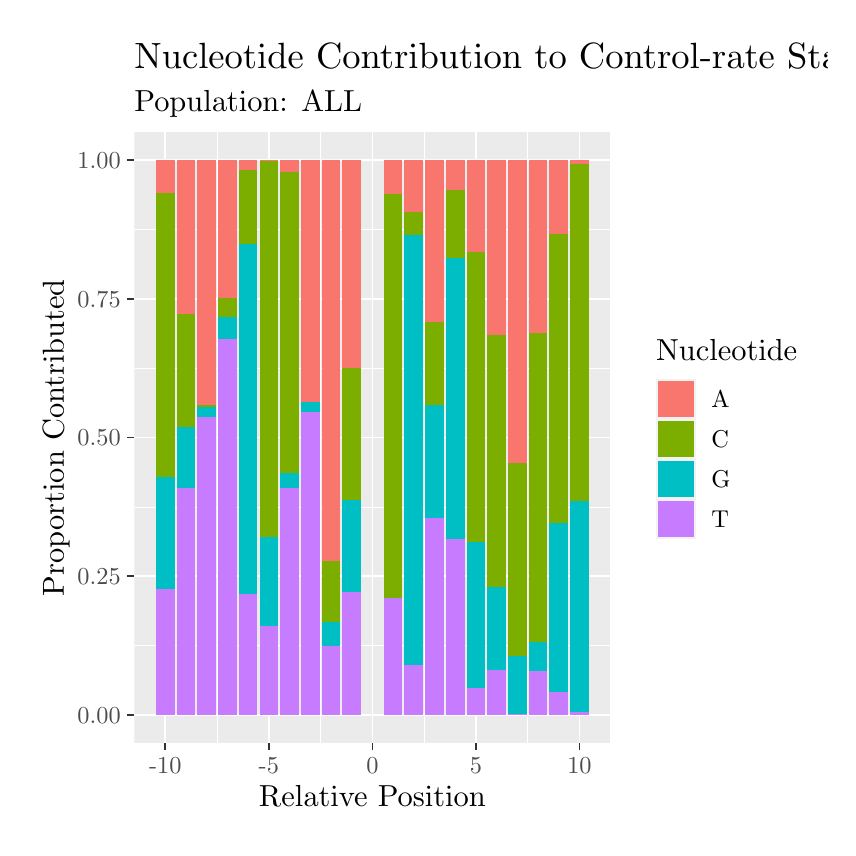
\begin{tikzpicture}[x=1pt,y=1pt]
\definecolor{fillColor}{RGB}{255,255,255}
\path[use as bounding box,fill=fillColor,fill opacity=0.00] (0,0) rectangle (289.08,289.08);
\begin{scope}
\path[clip] (  0.00,  0.00) rectangle (289.08,289.08);
\definecolor{drawColor}{RGB}{255,255,255}
\definecolor{fillColor}{RGB}{255,255,255}

\path[draw=drawColor,line width= 0.6pt,line join=round,line cap=round,fill=fillColor] (  0.00,  0.00) rectangle (289.08,289.08);
\end{scope}
\begin{scope}
\path[clip] ( 38.56, 30.69) rectangle (210.56,251.21);
\definecolor{fillColor}{gray}{0.92}

\path[fill=fillColor] ( 38.56, 30.69) rectangle (210.56,251.21);
\definecolor{drawColor}{RGB}{255,255,255}

\path[draw=drawColor,line width= 0.3pt,line join=round] ( 38.56, 65.77) --
	(210.56, 65.77);

\path[draw=drawColor,line width= 0.3pt,line join=round] ( 38.56,115.89) --
	(210.56,115.89);

\path[draw=drawColor,line width= 0.3pt,line join=round] ( 38.56,166.01) --
	(210.56,166.01);

\path[draw=drawColor,line width= 0.3pt,line join=round] ( 38.56,216.13) --
	(210.56,216.13);

\path[draw=drawColor,line width= 0.3pt,line join=round] ( 68.45, 30.69) --
	( 68.45,251.21);

\path[draw=drawColor,line width= 0.3pt,line join=round] (105.85, 30.69) --
	(105.85,251.21);

\path[draw=drawColor,line width= 0.3pt,line join=round] (143.26, 30.69) --
	(143.26,251.21);

\path[draw=drawColor,line width= 0.3pt,line join=round] (180.67, 30.69) --
	(180.67,251.21);

\path[draw=drawColor,line width= 0.6pt,line join=round] ( 38.56, 40.71) --
	(210.56, 40.71);

\path[draw=drawColor,line width= 0.6pt,line join=round] ( 38.56, 90.83) --
	(210.56, 90.83);

\path[draw=drawColor,line width= 0.6pt,line join=round] ( 38.56,140.95) --
	(210.56,140.95);

\path[draw=drawColor,line width= 0.6pt,line join=round] ( 38.56,191.07) --
	(210.56,191.07);

\path[draw=drawColor,line width= 0.6pt,line join=round] ( 38.56,241.18) --
	(210.56,241.18);

\path[draw=drawColor,line width= 0.6pt,line join=round] ( 49.74, 30.69) --
	( 49.74,251.21);

\path[draw=drawColor,line width= 0.6pt,line join=round] ( 87.15, 30.69) --
	( 87.15,251.21);

\path[draw=drawColor,line width= 0.6pt,line join=round] (124.56, 30.69) --
	(124.56,251.21);

\path[draw=drawColor,line width= 0.6pt,line join=round] (161.97, 30.69) --
	(161.97,251.21);

\path[draw=drawColor,line width= 0.6pt,line join=round] (199.38, 30.69) --
	(199.38,251.21);
\definecolor{fillColor}{RGB}{248,118,109}

\path[fill=fillColor] ( 46.37,229.19) rectangle ( 53.11,241.18);
\definecolor{fillColor}{RGB}{124,174,0}

\path[fill=fillColor] ( 46.37,126.81) rectangle ( 53.11,229.19);
\definecolor{fillColor}{RGB}{199,124,255}

\path[fill=fillColor] ( 46.37, 40.71) rectangle ( 53.11, 86.32);
\definecolor{fillColor}{RGB}{0,191,196}

\path[fill=fillColor] ( 46.37, 86.32) rectangle ( 53.11,126.81);
\definecolor{fillColor}{RGB}{248,118,109}

\path[fill=fillColor] ( 53.86,185.65) rectangle ( 60.59,241.18);
\definecolor{fillColor}{RGB}{124,174,0}

\path[fill=fillColor] ( 53.86,144.73) rectangle ( 60.59,185.65);
\definecolor{fillColor}{RGB}{199,124,255}

\path[fill=fillColor] ( 53.86, 40.71) rectangle ( 60.59,122.82);
\definecolor{fillColor}{RGB}{0,191,196}

\path[fill=fillColor] ( 53.86,122.82) rectangle ( 60.59,144.73);
\definecolor{fillColor}{RGB}{248,118,109}

\path[fill=fillColor] ( 61.34,152.63) rectangle ( 68.07,241.18);
\definecolor{fillColor}{RGB}{124,174,0}

\path[fill=fillColor] ( 61.34,152.15) rectangle ( 68.07,152.63);
\definecolor{fillColor}{RGB}{199,124,255}

\path[fill=fillColor] ( 61.34, 40.71) rectangle ( 68.07,148.22);
\definecolor{fillColor}{RGB}{0,191,196}

\path[fill=fillColor] ( 61.34,148.22) rectangle ( 68.07,152.15);
\definecolor{fillColor}{RGB}{248,118,109}

\path[fill=fillColor] ( 68.82,191.34) rectangle ( 75.55,241.18);
\definecolor{fillColor}{RGB}{124,174,0}

\path[fill=fillColor] ( 68.82,184.57) rectangle ( 75.55,191.34);
\definecolor{fillColor}{RGB}{0,191,196}

\path[fill=fillColor] ( 68.82,176.53) rectangle ( 75.55,184.57);
\definecolor{fillColor}{RGB}{199,124,255}

\path[fill=fillColor] ( 68.82, 40.71) rectangle ( 75.55,176.53);
\definecolor{fillColor}{RGB}{248,118,109}

\path[fill=fillColor] ( 76.30,237.65) rectangle ( 83.04,241.18);
\definecolor{fillColor}{RGB}{124,174,0}

\path[fill=fillColor] ( 76.30,210.87) rectangle ( 83.04,237.65);
\definecolor{fillColor}{RGB}{199,124,255}

\path[fill=fillColor] ( 76.30, 40.71) rectangle ( 83.04, 84.33);
\definecolor{fillColor}{RGB}{0,191,196}

\path[fill=fillColor] ( 76.30, 84.33) rectangle ( 83.04,210.87);
\definecolor{fillColor}{RGB}{248,118,109}

\path[fill=fillColor] ( 83.78,240.90) rectangle ( 90.52,241.18);
\definecolor{fillColor}{RGB}{124,174,0}

\path[fill=fillColor] ( 83.78,105.14) rectangle ( 90.52,240.90);
\definecolor{fillColor}{RGB}{199,124,255}

\path[fill=fillColor] ( 83.78, 40.71) rectangle ( 90.52, 72.83);
\definecolor{fillColor}{RGB}{0,191,196}

\path[fill=fillColor] ( 83.78, 72.83) rectangle ( 90.52,105.14);
\definecolor{fillColor}{RGB}{248,118,109}

\path[fill=fillColor] ( 91.27,236.75) rectangle ( 98.00,241.18);
\definecolor{fillColor}{RGB}{124,174,0}

\path[fill=fillColor] ( 91.27,128.08) rectangle ( 98.00,236.75);
\definecolor{fillColor}{RGB}{199,124,255}

\path[fill=fillColor] ( 91.27, 40.71) rectangle ( 98.00,122.72);
\definecolor{fillColor}{RGB}{0,191,196}

\path[fill=fillColor] ( 91.27,122.72) rectangle ( 98.00,128.08);
\definecolor{fillColor}{RGB}{248,118,109}

\path[fill=fillColor] ( 98.75,153.76) rectangle (105.48,241.18);
\definecolor{fillColor}{RGB}{124,174,0}

\path[fill=fillColor] ( 98.75,153.71) rectangle (105.48,153.76);
\definecolor{fillColor}{RGB}{199,124,255}

\path[fill=fillColor] ( 98.75, 40.71) rectangle (105.48,150.14);
\definecolor{fillColor}{RGB}{0,191,196}

\path[fill=fillColor] ( 98.75,150.14) rectangle (105.48,153.71);
\definecolor{fillColor}{RGB}{248,118,109}

\path[fill=fillColor] (106.23, 96.31) rectangle (112.96,241.18);
\definecolor{fillColor}{RGB}{124,174,0}

\path[fill=fillColor] (106.23, 74.27) rectangle (112.96, 96.31);
\definecolor{fillColor}{RGB}{0,191,196}

\path[fill=fillColor] (106.23, 65.60) rectangle (112.96, 74.27);
\definecolor{fillColor}{RGB}{199,124,255}

\path[fill=fillColor] (106.23, 40.71) rectangle (112.96, 65.60);
\definecolor{fillColor}{RGB}{248,118,109}

\path[fill=fillColor] (113.71,166.16) rectangle (120.44,241.18);
\definecolor{fillColor}{RGB}{124,174,0}

\path[fill=fillColor] (113.71,118.47) rectangle (120.44,166.16);
\definecolor{fillColor}{RGB}{199,124,255}

\path[fill=fillColor] (113.71, 40.71) rectangle (120.44, 85.01);
\definecolor{fillColor}{RGB}{0,191,196}

\path[fill=fillColor] (113.71, 85.01) rectangle (120.44,118.47);
\definecolor{fillColor}{RGB}{248,118,109}

\path[fill=fillColor] (128.67,229.15) rectangle (135.41,241.18);
\definecolor{fillColor}{RGB}{124,174,0}

\path[fill=fillColor] (128.67, 82.86) rectangle (135.41,229.15);
\definecolor{fillColor}{RGB}{199,124,255}

\path[fill=fillColor] (128.67, 40.71) rectangle (135.41, 82.86);
\definecolor{fillColor}{RGB}{0,191,196}

\path[fill=fillColor] (128.67, 82.86) rectangle (135.41, 82.86);
\definecolor{fillColor}{RGB}{248,118,109}

\path[fill=fillColor] (136.16,222.62) rectangle (142.89,241.18);
\definecolor{fillColor}{RGB}{124,174,0}

\path[fill=fillColor] (136.16,214.20) rectangle (142.89,222.62);
\definecolor{fillColor}{RGB}{0,191,196}

\path[fill=fillColor] (136.16, 58.87) rectangle (142.89,214.20);
\definecolor{fillColor}{RGB}{199,124,255}

\path[fill=fillColor] (136.16, 40.71) rectangle (142.89, 58.87);
\definecolor{fillColor}{RGB}{248,118,109}

\path[fill=fillColor] (143.64,182.87) rectangle (150.37,241.18);
\definecolor{fillColor}{RGB}{124,174,0}

\path[fill=fillColor] (143.64,152.88) rectangle (150.37,182.87);
\definecolor{fillColor}{RGB}{0,191,196}

\path[fill=fillColor] (143.64,111.89) rectangle (150.37,152.88);
\definecolor{fillColor}{RGB}{199,124,255}

\path[fill=fillColor] (143.64, 40.71) rectangle (150.37,111.89);
\definecolor{fillColor}{RGB}{248,118,109}

\path[fill=fillColor] (151.12,230.35) rectangle (157.85,241.18);
\definecolor{fillColor}{RGB}{124,174,0}

\path[fill=fillColor] (151.12,205.98) rectangle (157.85,230.35);
\definecolor{fillColor}{RGB}{0,191,196}

\path[fill=fillColor] (151.12,104.23) rectangle (157.85,205.98);
\definecolor{fillColor}{RGB}{199,124,255}

\path[fill=fillColor] (151.12, 40.71) rectangle (157.85,104.23);
\definecolor{fillColor}{RGB}{248,118,109}

\path[fill=fillColor] (158.60,208.01) rectangle (165.34,241.18);
\definecolor{fillColor}{RGB}{124,174,0}

\path[fill=fillColor] (158.60,103.32) rectangle (165.34,208.01);
\definecolor{fillColor}{RGB}{199,124,255}

\path[fill=fillColor] (158.60, 40.71) rectangle (165.34, 50.59);
\definecolor{fillColor}{RGB}{0,191,196}

\path[fill=fillColor] (158.60, 50.59) rectangle (165.34,103.32);
\definecolor{fillColor}{RGB}{248,118,109}

\path[fill=fillColor] (166.08,177.98) rectangle (172.82,241.18);
\definecolor{fillColor}{RGB}{124,174,0}

\path[fill=fillColor] (166.08, 87.14) rectangle (172.82,177.98);
\definecolor{fillColor}{RGB}{0,191,196}

\path[fill=fillColor] (166.08, 57.03) rectangle (172.82, 87.14);
\definecolor{fillColor}{RGB}{199,124,255}

\path[fill=fillColor] (166.08, 40.71) rectangle (172.82, 57.03);
\definecolor{fillColor}{RGB}{248,118,109}

\path[fill=fillColor] (173.57,131.73) rectangle (180.30,241.18);
\definecolor{fillColor}{RGB}{124,174,0}

\path[fill=fillColor] (173.57, 62.17) rectangle (180.30,131.73);
\definecolor{fillColor}{RGB}{199,124,255}

\path[fill=fillColor] (173.57, 40.71) rectangle (180.30, 41.09);
\definecolor{fillColor}{RGB}{0,191,196}

\path[fill=fillColor] (173.57, 41.09) rectangle (180.30, 62.17);
\definecolor{fillColor}{RGB}{248,118,109}

\path[fill=fillColor] (181.05,178.72) rectangle (187.78,241.18);
\definecolor{fillColor}{RGB}{124,174,0}

\path[fill=fillColor] (181.05, 67.19) rectangle (187.78,178.72);
\definecolor{fillColor}{RGB}{0,191,196}

\path[fill=fillColor] (181.05, 56.61) rectangle (187.78, 67.19);
\definecolor{fillColor}{RGB}{199,124,255}

\path[fill=fillColor] (181.05, 40.71) rectangle (187.78, 56.61);
\definecolor{fillColor}{RGB}{248,118,109}

\path[fill=fillColor] (188.53,214.54) rectangle (195.26,241.18);
\definecolor{fillColor}{RGB}{124,174,0}

\path[fill=fillColor] (188.53,110.16) rectangle (195.26,214.54);
\definecolor{fillColor}{RGB}{199,124,255}

\path[fill=fillColor] (188.53, 40.71) rectangle (195.26, 49.06);
\definecolor{fillColor}{RGB}{0,191,196}

\path[fill=fillColor] (188.53, 49.06) rectangle (195.26,110.16);
\definecolor{fillColor}{RGB}{248,118,109}

\path[fill=fillColor] (196.01,239.89) rectangle (202.75,241.18);
\definecolor{fillColor}{RGB}{124,174,0}

\path[fill=fillColor] (196.01,118.12) rectangle (202.75,239.89);
\definecolor{fillColor}{RGB}{0,191,196}

\path[fill=fillColor] (196.01, 41.66) rectangle (202.75,118.12);
\definecolor{fillColor}{RGB}{199,124,255}

\path[fill=fillColor] (196.01, 40.71) rectangle (202.75, 41.66);
\end{scope}
\begin{scope}
\path[clip] (  0.00,  0.00) rectangle (289.08,289.08);
\definecolor{drawColor}{gray}{0.30}

\node[text=drawColor,anchor=base east,inner sep=0pt, outer sep=0pt, scale=  0.88] at ( 33.61, 37.68) {0.00};

\node[text=drawColor,anchor=base east,inner sep=0pt, outer sep=0pt, scale=  0.88] at ( 33.61, 87.80) {0.25};

\node[text=drawColor,anchor=base east,inner sep=0pt, outer sep=0pt, scale=  0.88] at ( 33.61,137.92) {0.50};

\node[text=drawColor,anchor=base east,inner sep=0pt, outer sep=0pt, scale=  0.88] at ( 33.61,188.04) {0.75};

\node[text=drawColor,anchor=base east,inner sep=0pt, outer sep=0pt, scale=  0.88] at ( 33.61,238.15) {1.00};
\end{scope}
\begin{scope}
\path[clip] (  0.00,  0.00) rectangle (289.08,289.08);
\definecolor{drawColor}{gray}{0.20}

\path[draw=drawColor,line width= 0.6pt,line join=round] ( 35.81, 40.71) --
	( 38.56, 40.71);

\path[draw=drawColor,line width= 0.6pt,line join=round] ( 35.81, 90.83) --
	( 38.56, 90.83);

\path[draw=drawColor,line width= 0.6pt,line join=round] ( 35.81,140.95) --
	( 38.56,140.95);

\path[draw=drawColor,line width= 0.6pt,line join=round] ( 35.81,191.07) --
	( 38.56,191.07);

\path[draw=drawColor,line width= 0.6pt,line join=round] ( 35.81,241.18) --
	( 38.56,241.18);
\end{scope}
\begin{scope}
\path[clip] (  0.00,  0.00) rectangle (289.08,289.08);
\definecolor{drawColor}{gray}{0.20}

\path[draw=drawColor,line width= 0.6pt,line join=round] ( 49.74, 27.94) --
	( 49.74, 30.69);

\path[draw=drawColor,line width= 0.6pt,line join=round] ( 87.15, 27.94) --
	( 87.15, 30.69);

\path[draw=drawColor,line width= 0.6pt,line join=round] (124.56, 27.94) --
	(124.56, 30.69);

\path[draw=drawColor,line width= 0.6pt,line join=round] (161.97, 27.94) --
	(161.97, 30.69);

\path[draw=drawColor,line width= 0.6pt,line join=round] (199.38, 27.94) --
	(199.38, 30.69);
\end{scope}
\begin{scope}
\path[clip] (  0.00,  0.00) rectangle (289.08,289.08);
\definecolor{drawColor}{gray}{0.30}

\node[text=drawColor,anchor=base,inner sep=0pt, outer sep=0pt, scale=  0.88] at ( 49.74, 19.68) {-10};

\node[text=drawColor,anchor=base,inner sep=0pt, outer sep=0pt, scale=  0.88] at ( 87.15, 19.68) {-5};

\node[text=drawColor,anchor=base,inner sep=0pt, outer sep=0pt, scale=  0.88] at (124.56, 19.68) {0};

\node[text=drawColor,anchor=base,inner sep=0pt, outer sep=0pt, scale=  0.88] at (161.97, 19.68) {5};

\node[text=drawColor,anchor=base,inner sep=0pt, outer sep=0pt, scale=  0.88] at (199.38, 19.68) {10};
\end{scope}
\begin{scope}
\path[clip] (  0.00,  0.00) rectangle (289.08,289.08);
\definecolor{drawColor}{RGB}{0,0,0}

\node[text=drawColor,anchor=base,inner sep=0pt, outer sep=0pt, scale=  1.10] at (124.56,  7.64) {Relative Position};
\end{scope}
\begin{scope}
\path[clip] (  0.00,  0.00) rectangle (289.08,289.08);
\definecolor{drawColor}{RGB}{0,0,0}

\node[text=drawColor,rotate= 90.00,anchor=base,inner sep=0pt, outer sep=0pt, scale=  1.10] at ( 13.08,140.95) {Proportion Contributed};
\end{scope}
\begin{scope}
\path[clip] (  0.00,  0.00) rectangle (289.08,289.08);
\definecolor{fillColor}{RGB}{255,255,255}

\path[fill=fillColor] (221.56, 98.93) rectangle (283.58,182.96);
\end{scope}
\begin{scope}
\path[clip] (  0.00,  0.00) rectangle (289.08,289.08);
\definecolor{drawColor}{RGB}{0,0,0}

\node[text=drawColor,anchor=base west,inner sep=0pt, outer sep=0pt, scale=  1.10] at (227.06,168.82) {Nucleotide};
\end{scope}
\begin{scope}
\path[clip] (  0.00,  0.00) rectangle (289.08,289.08);
\definecolor{fillColor}{gray}{0.95}

\path[fill=fillColor] (227.06,147.79) rectangle (241.52,162.25);
\end{scope}
\begin{scope}
\path[clip] (  0.00,  0.00) rectangle (289.08,289.08);
\definecolor{fillColor}{RGB}{248,118,109}

\path[fill=fillColor] (227.78,148.51) rectangle (240.81,161.54);
\end{scope}
\begin{scope}
\path[clip] (  0.00,  0.00) rectangle (289.08,289.08);
\definecolor{fillColor}{gray}{0.95}

\path[fill=fillColor] (227.06,133.34) rectangle (241.52,147.79);
\end{scope}
\begin{scope}
\path[clip] (  0.00,  0.00) rectangle (289.08,289.08);
\definecolor{fillColor}{RGB}{124,174,0}

\path[fill=fillColor] (227.78,134.05) rectangle (240.81,147.08);
\end{scope}
\begin{scope}
\path[clip] (  0.00,  0.00) rectangle (289.08,289.08);
\definecolor{fillColor}{gray}{0.95}

\path[fill=fillColor] (227.06,118.89) rectangle (241.52,133.34);
\end{scope}
\begin{scope}
\path[clip] (  0.00,  0.00) rectangle (289.08,289.08);
\definecolor{fillColor}{RGB}{0,191,196}

\path[fill=fillColor] (227.78,119.60) rectangle (240.81,132.63);
\end{scope}
\begin{scope}
\path[clip] (  0.00,  0.00) rectangle (289.08,289.08);
\definecolor{fillColor}{gray}{0.95}

\path[fill=fillColor] (227.06,104.43) rectangle (241.52,118.89);
\end{scope}
\begin{scope}
\path[clip] (  0.00,  0.00) rectangle (289.08,289.08);
\definecolor{fillColor}{RGB}{199,124,255}

\path[fill=fillColor] (227.78,105.14) rectangle (240.81,118.17);
\end{scope}
\begin{scope}
\path[clip] (  0.00,  0.00) rectangle (289.08,289.08);
\definecolor{drawColor}{RGB}{0,0,0}

\node[text=drawColor,anchor=base west,inner sep=0pt, outer sep=0pt, scale=  0.88] at (247.02,151.99) {A};
\end{scope}
\begin{scope}
\path[clip] (  0.00,  0.00) rectangle (289.08,289.08);
\definecolor{drawColor}{RGB}{0,0,0}

\node[text=drawColor,anchor=base west,inner sep=0pt, outer sep=0pt, scale=  0.88] at (247.02,137.54) {C};
\end{scope}
\begin{scope}
\path[clip] (  0.00,  0.00) rectangle (289.08,289.08);
\definecolor{drawColor}{RGB}{0,0,0}

\node[text=drawColor,anchor=base west,inner sep=0pt, outer sep=0pt, scale=  0.88] at (247.02,123.08) {G};
\end{scope}
\begin{scope}
\path[clip] (  0.00,  0.00) rectangle (289.08,289.08);
\definecolor{drawColor}{RGB}{0,0,0}

\node[text=drawColor,anchor=base west,inner sep=0pt, outer sep=0pt, scale=  0.88] at (247.02,108.63) {T};
\end{scope}
\begin{scope}
\path[clip] (  0.00,  0.00) rectangle (289.08,289.08);
\definecolor{drawColor}{RGB}{0,0,0}

\node[text=drawColor,anchor=base west,inner sep=0pt, outer sep=0pt, scale=  1.10] at ( 38.56,258.85) {Population: ALL};
\end{scope}
\begin{scope}
\path[clip] (  0.00,  0.00) rectangle (289.08,289.08);
\definecolor{drawColor}{RGB}{0,0,0}

\node[text=drawColor,anchor=base west,inner sep=0pt, outer sep=0pt, scale=  1.32] at ( 38.56,274.49) {Nucleotide Contribution to Control-rate Statistic: GC-TA};
\end{scope}
\end{tikzpicture}
